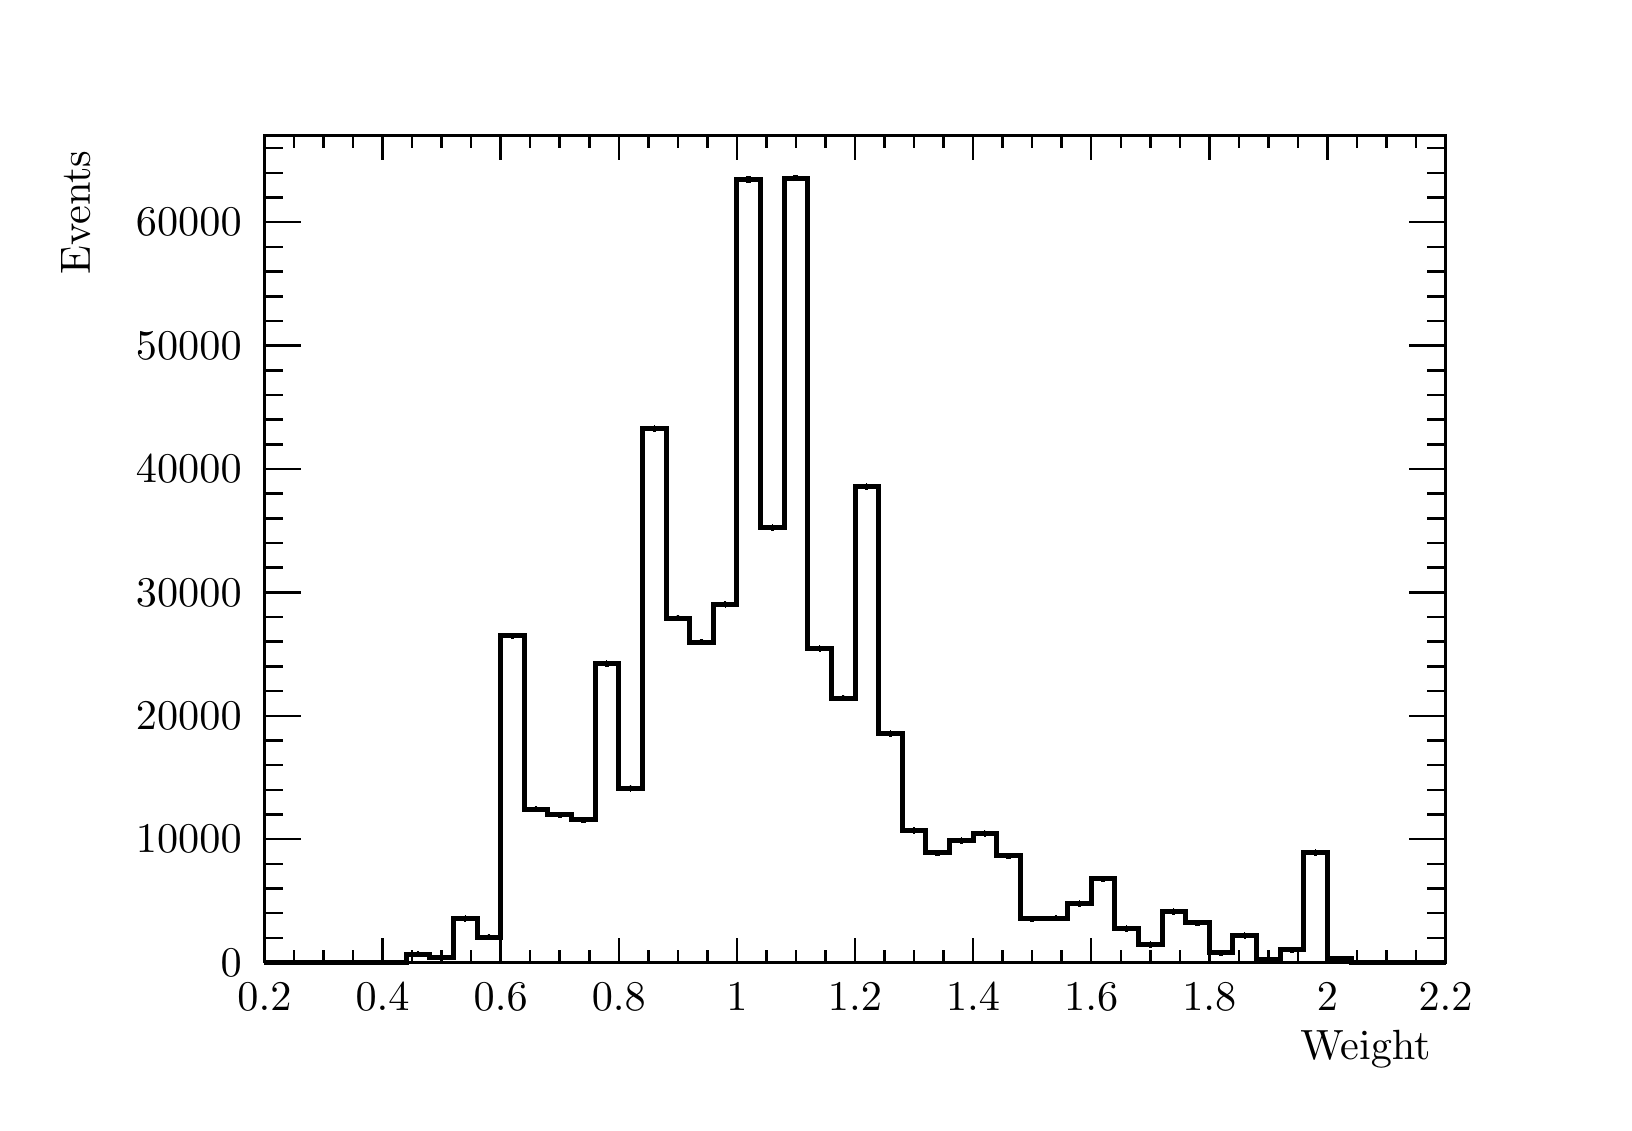
\begin{tikzpicture}
\pgfdeclareplotmark{cross} {
\pgfpathmoveto{\pgfpoint{-0.3\pgfplotmarksize}{\pgfplotmarksize}}
\pgfpathlineto{\pgfpoint{+0.3\pgfplotmarksize}{\pgfplotmarksize}}
\pgfpathlineto{\pgfpoint{+0.3\pgfplotmarksize}{0.3\pgfplotmarksize}}
\pgfpathlineto{\pgfpoint{+1\pgfplotmarksize}{0.3\pgfplotmarksize}}
\pgfpathlineto{\pgfpoint{+1\pgfplotmarksize}{-0.3\pgfplotmarksize}}
\pgfpathlineto{\pgfpoint{+0.3\pgfplotmarksize}{-0.3\pgfplotmarksize}}
\pgfpathlineto{\pgfpoint{+0.3\pgfplotmarksize}{-1.\pgfplotmarksize}}
\pgfpathlineto{\pgfpoint{-0.3\pgfplotmarksize}{-1.\pgfplotmarksize}}
\pgfpathlineto{\pgfpoint{-0.3\pgfplotmarksize}{-0.3\pgfplotmarksize}}
\pgfpathlineto{\pgfpoint{-1.\pgfplotmarksize}{-0.3\pgfplotmarksize}}
\pgfpathlineto{\pgfpoint{-1.\pgfplotmarksize}{0.3\pgfplotmarksize}}
\pgfpathlineto{\pgfpoint{-0.3\pgfplotmarksize}{0.3\pgfplotmarksize}}
\pgfpathclose
\pgfusepathqstroke
}
\pgfdeclareplotmark{cross*} {
\pgfpathmoveto{\pgfpoint{-0.3\pgfplotmarksize}{\pgfplotmarksize}}
\pgfpathlineto{\pgfpoint{+0.3\pgfplotmarksize}{\pgfplotmarksize}}
\pgfpathlineto{\pgfpoint{+0.3\pgfplotmarksize}{0.3\pgfplotmarksize}}
\pgfpathlineto{\pgfpoint{+1\pgfplotmarksize}{0.3\pgfplotmarksize}}
\pgfpathlineto{\pgfpoint{+1\pgfplotmarksize}{-0.3\pgfplotmarksize}}
\pgfpathlineto{\pgfpoint{+0.3\pgfplotmarksize}{-0.3\pgfplotmarksize}}
\pgfpathlineto{\pgfpoint{+0.3\pgfplotmarksize}{-1.\pgfplotmarksize}}
\pgfpathlineto{\pgfpoint{-0.3\pgfplotmarksize}{-1.\pgfplotmarksize}}
\pgfpathlineto{\pgfpoint{-0.3\pgfplotmarksize}{-0.3\pgfplotmarksize}}
\pgfpathlineto{\pgfpoint{-1.\pgfplotmarksize}{-0.3\pgfplotmarksize}}
\pgfpathlineto{\pgfpoint{-1.\pgfplotmarksize}{0.3\pgfplotmarksize}}
\pgfpathlineto{\pgfpoint{-0.3\pgfplotmarksize}{0.3\pgfplotmarksize}}
\pgfpathclose
\pgfusepathqfillstroke
}
\pgfdeclareplotmark{newstar} {
\pgfpathmoveto{\pgfqpoint{0pt}{\pgfplotmarksize}}
\pgfpathlineto{\pgfqpointpolar{44}{0.5\pgfplotmarksize}}
\pgfpathlineto{\pgfqpointpolar{18}{\pgfplotmarksize}}
\pgfpathlineto{\pgfqpointpolar{-20}{0.5\pgfplotmarksize}}
\pgfpathlineto{\pgfqpointpolar{-54}{\pgfplotmarksize}}
\pgfpathlineto{\pgfqpointpolar{-90}{0.5\pgfplotmarksize}}
\pgfpathlineto{\pgfqpointpolar{234}{\pgfplotmarksize}}
\pgfpathlineto{\pgfqpointpolar{198}{0.5\pgfplotmarksize}}
\pgfpathlineto{\pgfqpointpolar{162}{\pgfplotmarksize}}
\pgfpathlineto{\pgfqpointpolar{134}{0.5\pgfplotmarksize}}
\pgfpathclose
\pgfusepathqstroke
}
\pgfdeclareplotmark{newstar*} {
\pgfpathmoveto{\pgfqpoint{0pt}{\pgfplotmarksize}}
\pgfpathlineto{\pgfqpointpolar{44}{0.5\pgfplotmarksize}}
\pgfpathlineto{\pgfqpointpolar{18}{\pgfplotmarksize}}
\pgfpathlineto{\pgfqpointpolar{-20}{0.5\pgfplotmarksize}}
\pgfpathlineto{\pgfqpointpolar{-54}{\pgfplotmarksize}}
\pgfpathlineto{\pgfqpointpolar{-90}{0.5\pgfplotmarksize}}
\pgfpathlineto{\pgfqpointpolar{234}{\pgfplotmarksize}}
\pgfpathlineto{\pgfqpointpolar{198}{0.5\pgfplotmarksize}}
\pgfpathlineto{\pgfqpointpolar{162}{\pgfplotmarksize}}
\pgfpathlineto{\pgfqpointpolar{134}{0.5\pgfplotmarksize}}
\pgfpathclose
\pgfusepathqfillstroke
}
\definecolor{c}{rgb}{1,1,1};
\draw [color=c, fill=c] (0,0) rectangle (20,13.639);
\draw [color=c, fill=c] (3,1.77307) rectangle (18,12.2751);
\definecolor{c}{rgb}{0,0,0};
\draw [c,line width=0.9] (3,1.77307) -- (3,12.2751) -- (18,12.2751) -- (18,1.77307) -- (3,1.77307);
\definecolor{c}{rgb}{1,1,1};
\draw [color=c, fill=c] (3,1.77307) rectangle (18,12.2751);
\definecolor{c}{rgb}{0,0,0};
\draw [c,line width=0.9] (3,1.77307) -- (3,12.2751) -- (18,12.2751) -- (18,1.77307) -- (3,1.77307);
\draw [c,line width=1.8] (4.95,1.87523) -- (4.95,1.87931);
\draw [c,line width=1.8] (4.95,1.87931) -- (4.95,1.88339);
\foreach \P in {(4.95,1.87931)}{\draw[mark options={color=c,fill=c},mark size=2.402402pt, line width=0.000000pt, mark=*,mark size=1pt] plot coordinates {\P};}
\draw [c,line width=1.8] (5.25,1.83063) -- (5.25,1.83371);
\draw [c,line width=1.8] (5.25,1.83371) -- (5.25,1.83679);
\foreach \P in {(5.25,1.83371)}{\draw[mark options={color=c,fill=c},mark size=2.402402pt, line width=0.000000pt, mark=*,mark size=1pt] plot coordinates {\P};}
\draw [c,line width=1.8] (5.55,2.32328) -- (5.55,2.33264);
\draw [c,line width=1.8] (5.55,2.33264) -- (5.55,2.34201);
\foreach \P in {(5.55,2.33264)}{\draw[mark options={color=c,fill=c},mark size=2.402402pt, line width=0.000000pt, mark=*,mark size=1pt] plot coordinates {\P};}
\draw [c,line width=1.8] (5.85,2.08845) -- (5.85,2.09556);
\draw [c,line width=1.8] (5.85,2.09556) -- (5.85,2.10266);
\foreach \P in {(5.85,2.09556)}{\draw[mark options={color=c,fill=c},mark size=2.402402pt, line width=0.000000pt, mark=*,mark size=1pt] plot coordinates {\P};}
\draw [c,line width=1.8] (6.15,5.897) -- (6.15,5.9225);
\draw [c,line width=1.8] (6.15,5.9225) -- (6.15,5.948);
\foreach \P in {(6.15,5.9225)}{\draw[mark options={color=c,fill=c},mark size=2.402402pt, line width=0.000000pt, mark=*,mark size=1pt] plot coordinates {\P};}
\draw [c,line width=1.8] (6.45,3.70323) -- (6.45,3.7207);
\draw [c,line width=1.8] (6.45,3.7207) -- (6.45,3.73817);
\foreach \P in {(6.45,3.7207)}{\draw[mark options={color=c,fill=c},mark size=2.402402pt, line width=0.000000pt, mark=*,mark size=1pt] plot coordinates {\P};}
\draw [c,line width=1.8] (6.75,3.63132) -- (6.75,3.64846);
\draw [c,line width=1.8] (6.75,3.64846) -- (6.75,3.6656);
\foreach \P in {(6.75,3.64846)}{\draw[mark options={color=c,fill=c},mark size=2.402402pt, line width=0.000000pt, mark=*,mark size=1pt] plot coordinates {\P};}
\draw [c,line width=1.8] (7.05,3.56674) -- (7.05,3.58359);
\draw [c,line width=1.8] (7.05,3.58359) -- (7.05,3.60043);
\foreach \P in {(7.05,3.58359)}{\draw[mark options={color=c,fill=c},mark size=2.402402pt, line width=0.000000pt, mark=*,mark size=1pt] plot coordinates {\P};}
\draw [c,line width=1.8] (7.35,5.54412) -- (7.35,5.56851);
\draw [c,line width=1.8] (7.35,5.56851) -- (7.35,5.5929);
\foreach \P in {(7.35,5.56851)}{\draw[mark options={color=c,fill=c},mark size=2.402402pt, line width=0.000000pt, mark=*,mark size=1pt] plot coordinates {\P};}
\draw [c,line width=1.8] (7.65,3.96799) -- (7.65,3.98662);
\draw [c,line width=1.8] (7.65,3.98662) -- (7.65,4.00524);
\foreach \P in {(7.65,3.98662)}{\draw[mark options={color=c,fill=c},mark size=2.402402pt, line width=0.000000pt, mark=*,mark size=1pt] plot coordinates {\P};}
\draw [c,line width=1.8] (7.95,8.52091) -- (7.95,8.5535);
\draw [c,line width=1.8] (7.95,8.5535) -- (7.95,8.5861);
\foreach \P in {(7.95,8.5535)}{\draw[mark options={color=c,fill=c},mark size=2.402402pt, line width=0.000000pt, mark=*,mark size=1pt] plot coordinates {\P};}
\draw [c,line width=1.8] (8.25,6.12243) -- (8.25,6.14862);
\draw [c,line width=1.8] (8.25,6.14862) -- (8.25,6.1748);
\foreach \P in {(8.25,6.14862)}{\draw[mark options={color=c,fill=c},mark size=2.402402pt, line width=0.000000pt, mark=*,mark size=1pt] plot coordinates {\P};}
\draw [c,line width=1.8] (8.55,5.81842) -- (8.55,5.84368);
\draw [c,line width=1.8] (8.55,5.84368) -- (8.55,5.86893);
\foreach \P in {(8.55,5.84368)}{\draw[mark options={color=c,fill=c},mark size=2.402402pt, line width=0.000000pt, mark=*,mark size=1pt] plot coordinates {\P};}
\draw [c,line width=1.8] (8.85,6.29679) -- (8.85,6.3235);
\draw [c,line width=1.8] (8.85,6.3235) -- (8.85,6.3502);
\foreach \P in {(8.85,6.3235)}{\draw[mark options={color=c,fill=c},mark size=2.402402pt, line width=0.000000pt, mark=*,mark size=1pt] plot coordinates {\P};}
\draw [c,line width=1.8] (9.15,11.6789) -- (9.15,11.7184);
\draw [c,line width=1.8] (9.15,11.7184) -- (9.15,11.7579);
\foreach \P in {(9.15,11.7184)}{\draw[mark options={color=c,fill=c},mark size=2.402402pt, line width=0.000000pt, mark=*,mark size=1pt] plot coordinates {\P};}
\draw [c,line width=1.8] (9.45,7.26703) -- (9.45,7.29645);
\draw [c,line width=1.8] (9.45,7.29645) -- (9.45,7.32587);
\foreach \P in {(9.45,7.29645)}{\draw[mark options={color=c,fill=c},mark size=2.402402pt, line width=0.000000pt, mark=*,mark size=1pt] plot coordinates {\P};}
\draw [c,line width=1.8] (9.75,11.696) -- (9.75,11.7355);
\draw [c,line width=1.8] (9.75,11.7355) -- (9.75,11.775);
\foreach \P in {(9.75,11.7355)}{\draw[mark options={color=c,fill=c},mark size=2.402402pt, line width=0.000000pt, mark=*,mark size=1pt] plot coordinates {\P};}
\draw [c,line width=1.8] (10.05,5.73719) -- (10.05,5.76219);
\draw [c,line width=1.8] (10.05,5.76219) -- (10.05,5.7872);
\foreach \P in {(10.05,5.76219)}{\draw[mark options={color=c,fill=c},mark size=2.402402pt, line width=0.000000pt, mark=*,mark size=1pt] plot coordinates {\P};}
\draw [c,line width=1.8] (10.35,5.10838) -- (10.35,5.13132);
\draw [c,line width=1.8] (10.35,5.13132) -- (10.35,5.15426);
\foreach \P in {(10.35,5.13132)}{\draw[mark options={color=c,fill=c},mark size=2.402402pt, line width=0.000000pt, mark=*,mark size=1pt] plot coordinates {\P};}
\draw [c,line width=1.8] (10.65,7.78702) -- (10.65,7.81779);
\draw [c,line width=1.8] (10.65,7.81779) -- (10.65,7.84857);
\foreach \P in {(10.65,7.81779)}{\draw[mark options={color=c,fill=c},mark size=2.402402pt, line width=0.000000pt, mark=*,mark size=1pt] plot coordinates {\P};}
\draw [c,line width=1.8] (10.95,4.65852) -- (10.95,4.67986);
\draw [c,line width=1.8] (10.95,4.67986) -- (10.95,4.7012);
\foreach \P in {(10.95,4.67986)}{\draw[mark options={color=c,fill=c},mark size=2.402402pt, line width=0.000000pt, mark=*,mark size=1pt] plot coordinates {\P};}
\draw [c,line width=1.8] (11.25,3.4362) -- (11.25,3.45243);
\draw [c,line width=1.8] (11.25,3.45243) -- (11.25,3.46865);
\foreach \P in {(11.25,3.45243)}{\draw[mark options={color=c,fill=c},mark size=2.402402pt, line width=0.000000pt, mark=*,mark size=1pt] plot coordinates {\P};}
\draw [c,line width=1.8] (11.55,3.15042) -- (11.55,3.16519);
\draw [c,line width=1.8] (11.55,3.16519) -- (11.55,3.17996);
\foreach \P in {(11.55,3.16519)}{\draw[mark options={color=c,fill=c},mark size=2.402402pt, line width=0.000000pt, mark=*,mark size=1pt] plot coordinates {\P};}
\draw [c,line width=1.8] (11.85,3.30663) -- (11.85,3.32221);
\draw [c,line width=1.8] (11.85,3.32221) -- (11.85,3.33779);
\foreach \P in {(11.85,3.32221)}{\draw[mark options={color=c,fill=c},mark size=2.402402pt, line width=0.000000pt, mark=*,mark size=1pt] plot coordinates {\P};}
\draw [c,line width=1.8] (12.15,3.39675) -- (12.15,3.41278);
\draw [c,line width=1.8] (12.15,3.41278) -- (12.15,3.42881);
\foreach \P in {(12.15,3.41278)}{\draw[mark options={color=c,fill=c},mark size=2.402402pt, line width=0.000000pt, mark=*,mark size=1pt] plot coordinates {\P};}
\draw [c,line width=1.8] (12.45,3.11271) -- (12.45,3.12727);
\draw [c,line width=1.8] (12.45,3.12727) -- (12.45,3.14184);
\foreach \P in {(12.45,3.12727)}{\draw[mark options={color=c,fill=c},mark size=2.402402pt, line width=0.000000pt, mark=*,mark size=1pt] plot coordinates {\P};}
\draw [c,line width=1.8] (12.75,2.31738) -- (12.75,2.32669);
\draw [c,line width=1.8] (12.75,2.32669) -- (12.75,2.336);
\foreach \P in {(12.75,2.32669)}{\draw[mark options={color=c,fill=c},mark size=2.402402pt, line width=0.000000pt, mark=*,mark size=1pt] plot coordinates {\P};}
\draw [c,line width=1.8] (13.05,2.32654) -- (13.05,2.33593);
\draw [c,line width=1.8] (13.05,2.33593) -- (13.05,2.34533);
\foreach \P in {(13.05,2.33593)}{\draw[mark options={color=c,fill=c},mark size=2.402402pt, line width=0.000000pt, mark=*,mark size=1pt] plot coordinates {\P};}
\draw [c,line width=1.8] (13.35,2.50986) -- (13.35,2.52068);
\draw [c,line width=1.8] (13.35,2.52068) -- (13.35,2.53151);
\foreach \P in {(13.35,2.52068)}{\draw[mark options={color=c,fill=c},mark size=2.402402pt, line width=0.000000pt, mark=*,mark size=1pt] plot coordinates {\P};}
\draw [c,line width=1.8] (13.65,2.82384) -- (13.65,2.83675);
\draw [c,line width=1.8] (13.65,2.83675) -- (13.65,2.84966);
\foreach \P in {(13.65,2.83675)}{\draw[mark options={color=c,fill=c},mark size=2.402402pt, line width=0.000000pt, mark=*,mark size=1pt] plot coordinates {\P};}
\draw [c,line width=1.8] (13.95,2.19671) -- (13.95,2.20493);
\draw [c,line width=1.8] (13.95,2.20493) -- (13.95,2.21316);
\foreach \P in {(13.95,2.20493)}{\draw[mark options={color=c,fill=c},mark size=2.402402pt, line width=0.000000pt, mark=*,mark size=1pt] plot coordinates {\P};}
\draw [c,line width=1.8] (14.25,1.99478) -- (14.25,2.00075);
\draw [c,line width=1.8] (14.25,2.00075) -- (14.25,2.00673);
\foreach \P in {(14.25,2.00075)}{\draw[mark options={color=c,fill=c},mark size=2.402402pt, line width=0.000000pt, mark=*,mark size=1pt] plot coordinates {\P};}
\draw [c,line width=1.8] (14.55,2.40986) -- (14.55,2.41993);
\draw [c,line width=1.8] (14.55,2.41993) -- (14.55,2.42999);
\foreach \P in {(14.55,2.41993)}{\draw[mark options={color=c,fill=c},mark size=2.402402pt, line width=0.000000pt, mark=*,mark size=1pt] plot coordinates {\P};}
\draw [c,line width=1.8] (14.85,2.26735) -- (14.85,2.27623);
\draw [c,line width=1.8] (14.85,2.27623) -- (14.85,2.28511);
\foreach \P in {(14.85,2.27623)}{\draw[mark options={color=c,fill=c},mark size=2.402402pt, line width=0.000000pt, mark=*,mark size=1pt] plot coordinates {\P};}
\draw [c,line width=1.8] (15.15,1.89107) -- (15.15,1.89545);
\draw [c,line width=1.8] (15.15,1.89545) -- (15.15,1.89983);
\foreach \P in {(15.15,1.89545)}{\draw[mark options={color=c,fill=c},mark size=2.402402pt, line width=0.000000pt, mark=*,mark size=1pt] plot coordinates {\P};}
\draw [c,line width=1.8] (15.45,2.10937) -- (15.45,2.11671);
\draw [c,line width=1.8] (15.45,2.11671) -- (15.45,2.12405);
\foreach \P in {(15.45,2.11671)}{\draw[mark options={color=c,fill=c},mark size=2.402402pt, line width=0.000000pt, mark=*,mark size=1pt] plot coordinates {\P};}
\draw [c,line width=1.8] (15.75,1.81052) -- (15.75,1.81302);
\draw [c,line width=1.8] (15.75,1.81302) -- (15.75,1.81553);
\foreach \P in {(15.75,1.81302)}{\draw[mark options={color=c,fill=c},mark size=2.402402pt, line width=0.000000pt, mark=*,mark size=1pt] plot coordinates {\P};}
\draw [c,line width=1.8] (16.05,1.92759) -- (16.05,1.93259);
\draw [c,line width=1.8] (16.05,1.93259) -- (16.05,1.93759);
\foreach \P in {(16.05,1.93259)}{\draw[mark options={color=c,fill=c},mark size=2.402402pt, line width=0.000000pt, mark=*,mark size=1pt] plot coordinates {\P};}
\draw [c,line width=1.8] (16.35,3.1551) -- (16.35,3.1699);
\draw [c,line width=1.8] (16.35,3.1699) -- (16.35,3.18469);
\foreach \P in {(16.35,3.1699)}{\draw[mark options={color=c,fill=c},mark size=2.402402pt, line width=0.000000pt, mark=*,mark size=1pt] plot coordinates {\P};}
\draw [c,line width=1.8] (16.65,1.81675) -- (16.65,1.81945);
\draw [c,line width=1.8] (16.65,1.81945) -- (16.65,1.82215);
\foreach \P in {(16.65,1.81945)}{\draw[mark options={color=c,fill=c},mark size=2.402402pt, line width=0.000000pt, mark=*,mark size=1pt] plot coordinates {\P};}
\draw [c,line width=1.8] (3,1.77307) -- (3.3,1.77307) -- (3.3,1.77307) -- (3.6,1.77307) -- (3.6,1.77307) -- (3.9,1.77307) -- (3.9,1.77307) -- (4.2,1.77307) -- (4.2,1.77307) -- (4.5,1.77307) -- (4.5,1.77307) -- (4.8,1.77307) -- (4.8,1.87931) --
 (5.1,1.87931) -- (5.1,1.83371) -- (5.4,1.83371) -- (5.4,2.33264) -- (5.7,2.33264) -- (5.7,2.09556) -- (6,2.09556) -- (6,5.9225) -- (6.3,5.9225) -- (6.3,3.7207) -- (6.6,3.7207) -- (6.6,3.64846) -- (6.9,3.64846) -- (6.9,3.58359) -- (7.2,3.58359) --
 (7.2,5.56851) -- (7.5,5.56851) -- (7.5,3.98662) -- (7.8,3.98662) -- (7.8,8.5535) -- (8.1,8.5535) -- (8.1,6.14862) -- (8.4,6.14862) -- (8.4,5.84368) -- (8.7,5.84368) -- (8.7,6.3235) -- (9,6.3235) -- (9,11.7184) -- (9.3,11.7184) -- (9.3,7.29645) --
 (9.6,7.29645) -- (9.6,11.7355) -- (9.9,11.7355) -- (9.9,5.76219) -- (10.2,5.76219) -- (10.2,5.13132) -- (10.5,5.13132) -- (10.5,7.81779) -- (10.8,7.81779) -- (10.8,4.67986) -- (11.1,4.67986) -- (11.1,3.45243) -- (11.4,3.45243) -- (11.4,3.16519) --
 (11.7,3.16519) -- (11.7,3.32221) -- (12,3.32221) -- (12,3.41278) -- (12.3,3.41278) -- (12.3,3.12727) -- (12.6,3.12727) -- (12.6,2.32669) -- (12.9,2.32669) -- (12.9,2.33593) -- (13.2,2.33593) -- (13.2,2.52068) -- (13.5,2.52068) -- (13.5,2.83675) --
 (13.8,2.83675) -- (13.8,2.20493) -- (14.1,2.20493) -- (14.1,2.00075) -- (14.4,2.00075) -- (14.4,2.41993) -- (14.7,2.41993) -- (14.7,2.27623) -- (15,2.27623) -- (15,1.89545) -- (15.3,1.89545) -- (15.3,2.11671) -- (15.6,2.11671) -- (15.6,1.81302) --
 (15.9,1.81302) -- (15.9,1.93259) -- (16.2,1.93259) -- (16.2,3.1699) -- (16.5,3.1699) -- (16.5,1.81945) -- (16.8,1.81945) -- (16.8,1.77307) -- (17.1,1.77307) -- (17.1,1.77307) -- (17.4,1.77307) -- (17.4,1.77307) -- (17.7,1.77307) -- (17.7,1.77307) --
 (18,1.77307);
\draw [c,line width=0.9] (3,1.77307) -- (18,1.77307);
\draw [c,line width=0.9] (3,2.07994) -- (3,1.77307);
\draw [c,line width=0.9] (3.375,1.9265) -- (3.375,1.77307);
\draw [c,line width=0.9] (3.75,1.9265) -- (3.75,1.77307);
\draw [c,line width=0.9] (4.125,1.9265) -- (4.125,1.77307);
\draw [c,line width=0.9] (4.5,2.07994) -- (4.5,1.77307);
\draw [c,line width=0.9] (4.875,1.9265) -- (4.875,1.77307);
\draw [c,line width=0.9] (5.25,1.9265) -- (5.25,1.77307);
\draw [c,line width=0.9] (5.625,1.9265) -- (5.625,1.77307);
\draw [c,line width=0.9] (6,2.07994) -- (6,1.77307);
\draw [c,line width=0.9] (6.375,1.9265) -- (6.375,1.77307);
\draw [c,line width=0.9] (6.75,1.9265) -- (6.75,1.77307);
\draw [c,line width=0.9] (7.125,1.9265) -- (7.125,1.77307);
\draw [c,line width=0.9] (7.5,2.07994) -- (7.5,1.77307);
\draw [c,line width=0.9] (7.875,1.9265) -- (7.875,1.77307);
\draw [c,line width=0.9] (8.25,1.9265) -- (8.25,1.77307);
\draw [c,line width=0.9] (8.625,1.9265) -- (8.625,1.77307);
\draw [c,line width=0.9] (9,2.07994) -- (9,1.77307);
\draw [c,line width=0.9] (9.375,1.9265) -- (9.375,1.77307);
\draw [c,line width=0.9] (9.75,1.9265) -- (9.75,1.77307);
\draw [c,line width=0.9] (10.125,1.9265) -- (10.125,1.77307);
\draw [c,line width=0.9] (10.5,2.07994) -- (10.5,1.77307);
\draw [c,line width=0.9] (10.875,1.9265) -- (10.875,1.77307);
\draw [c,line width=0.9] (11.25,1.9265) -- (11.25,1.77307);
\draw [c,line width=0.9] (11.625,1.9265) -- (11.625,1.77307);
\draw [c,line width=0.9] (12,2.07994) -- (12,1.77307);
\draw [c,line width=0.9] (12.375,1.9265) -- (12.375,1.77307);
\draw [c,line width=0.9] (12.75,1.9265) -- (12.75,1.77307);
\draw [c,line width=0.9] (13.125,1.9265) -- (13.125,1.77307);
\draw [c,line width=0.9] (13.5,2.07994) -- (13.5,1.77307);
\draw [c,line width=0.9] (13.875,1.9265) -- (13.875,1.77307);
\draw [c,line width=0.9] (14.25,1.9265) -- (14.25,1.77307);
\draw [c,line width=0.9] (14.625,1.9265) -- (14.625,1.77307);
\draw [c,line width=0.9] (15,2.07994) -- (15,1.77307);
\draw [c,line width=0.9] (15.375,1.9265) -- (15.375,1.77307);
\draw [c,line width=0.9] (15.75,1.9265) -- (15.75,1.77307);
\draw [c,line width=0.9] (16.125,1.9265) -- (16.125,1.77307);
\draw [c,line width=0.9] (16.5,2.07994) -- (16.5,1.77307);
\draw [c,line width=0.9] (16.875,1.9265) -- (16.875,1.77307);
\draw [c,line width=0.9] (17.25,1.9265) -- (17.25,1.77307);
\draw [c,line width=0.9] (17.625,1.9265) -- (17.625,1.77307);
\draw [c,line width=0.9] (18,2.07994) -- (18,1.77307);
\draw [anchor=base] (3,1.15931) node[scale=1.52731, color=c, rotate=0]{0.2};
\draw [anchor=base] (4.5,1.15931) node[scale=1.52731, color=c, rotate=0]{0.4};
\draw [anchor=base] (6,1.15931) node[scale=1.52731, color=c, rotate=0]{0.6};
\draw [anchor=base] (7.5,1.15931) node[scale=1.52731, color=c, rotate=0]{0.8};
\draw [anchor=base] (9,1.15931) node[scale=1.52731, color=c, rotate=0]{1};
\draw [anchor=base] (10.5,1.15931) node[scale=1.52731, color=c, rotate=0]{1.2};
\draw [anchor=base] (12,1.15931) node[scale=1.52731, color=c, rotate=0]{1.4};
\draw [anchor=base] (13.5,1.15931) node[scale=1.52731, color=c, rotate=0]{1.6};
\draw [anchor=base] (15,1.15931) node[scale=1.52731, color=c, rotate=0]{1.8};
\draw [anchor=base] (16.5,1.15931) node[scale=1.52731, color=c, rotate=0]{2};
\draw [anchor=base] (18,1.15931) node[scale=1.52731, color=c, rotate=0]{2.2};
\draw [anchor= east] (18,0.681948) node[scale=1.52731, color=c, rotate=0]{ Weight};
\draw [c,line width=0.9] (3,12.2751) -- (18,12.2751);
\draw [c,line width=0.9] (3,11.9682) -- (3,12.2751);
\draw [c,line width=0.9] (3.375,12.1216) -- (3.375,12.2751);
\draw [c,line width=0.9] (3.75,12.1216) -- (3.75,12.2751);
\draw [c,line width=0.9] (4.125,12.1216) -- (4.125,12.2751);
\draw [c,line width=0.9] (4.5,11.9682) -- (4.5,12.2751);
\draw [c,line width=0.9] (4.875,12.1216) -- (4.875,12.2751);
\draw [c,line width=0.9] (5.25,12.1216) -- (5.25,12.2751);
\draw [c,line width=0.9] (5.625,12.1216) -- (5.625,12.2751);
\draw [c,line width=0.9] (6,11.9682) -- (6,12.2751);
\draw [c,line width=0.9] (6.375,12.1216) -- (6.375,12.2751);
\draw [c,line width=0.9] (6.75,12.1216) -- (6.75,12.2751);
\draw [c,line width=0.9] (7.125,12.1216) -- (7.125,12.2751);
\draw [c,line width=0.9] (7.5,11.9682) -- (7.5,12.2751);
\draw [c,line width=0.9] (7.875,12.1216) -- (7.875,12.2751);
\draw [c,line width=0.9] (8.25,12.1216) -- (8.25,12.2751);
\draw [c,line width=0.9] (8.625,12.1216) -- (8.625,12.2751);
\draw [c,line width=0.9] (9,11.9682) -- (9,12.2751);
\draw [c,line width=0.9] (9.375,12.1216) -- (9.375,12.2751);
\draw [c,line width=0.9] (9.75,12.1216) -- (9.75,12.2751);
\draw [c,line width=0.9] (10.125,12.1216) -- (10.125,12.2751);
\draw [c,line width=0.9] (10.5,11.9682) -- (10.5,12.2751);
\draw [c,line width=0.9] (10.875,12.1216) -- (10.875,12.2751);
\draw [c,line width=0.9] (11.25,12.1216) -- (11.25,12.2751);
\draw [c,line width=0.9] (11.625,12.1216) -- (11.625,12.2751);
\draw [c,line width=0.9] (12,11.9682) -- (12,12.2751);
\draw [c,line width=0.9] (12.375,12.1216) -- (12.375,12.2751);
\draw [c,line width=0.9] (12.75,12.1216) -- (12.75,12.2751);
\draw [c,line width=0.9] (13.125,12.1216) -- (13.125,12.2751);
\draw [c,line width=0.9] (13.5,11.9682) -- (13.5,12.2751);
\draw [c,line width=0.9] (13.875,12.1216) -- (13.875,12.2751);
\draw [c,line width=0.9] (14.25,12.1216) -- (14.25,12.2751);
\draw [c,line width=0.9] (14.625,12.1216) -- (14.625,12.2751);
\draw [c,line width=0.9] (15,11.9682) -- (15,12.2751);
\draw [c,line width=0.9] (15.375,12.1216) -- (15.375,12.2751);
\draw [c,line width=0.9] (15.75,12.1216) -- (15.75,12.2751);
\draw [c,line width=0.9] (16.125,12.1216) -- (16.125,12.2751);
\draw [c,line width=0.9] (16.5,11.9682) -- (16.5,12.2751);
\draw [c,line width=0.9] (16.875,12.1216) -- (16.875,12.2751);
\draw [c,line width=0.9] (17.25,12.1216) -- (17.25,12.2751);
\draw [c,line width=0.9] (17.625,12.1216) -- (17.625,12.2751);
\draw [c,line width=0.9] (18,11.9682) -- (18,12.2751);
\draw [c,line width=0.9] (3,1.77307) -- (3,12.2751);
\draw [c,line width=0.9] (3.462,1.77307) -- (3,1.77307);
\draw [c,line width=0.9] (3.231,2.08647) -- (3,2.08647);
\draw [c,line width=0.9] (3.231,2.39987) -- (3,2.39987);
\draw [c,line width=0.9] (3.231,2.71327) -- (3,2.71327);
\draw [c,line width=0.9] (3.231,3.02667) -- (3,3.02667);
\draw [c,line width=0.9] (3.462,3.34007) -- (3,3.34007);
\draw [c,line width=0.9] (3.231,3.65347) -- (3,3.65347);
\draw [c,line width=0.9] (3.231,3.96687) -- (3,3.96687);
\draw [c,line width=0.9] (3.231,4.28028) -- (3,4.28028);
\draw [c,line width=0.9] (3.231,4.59368) -- (3,4.59368);
\draw [c,line width=0.9] (3.462,4.90708) -- (3,4.90708);
\draw [c,line width=0.9] (3.231,5.22048) -- (3,5.22048);
\draw [c,line width=0.9] (3.231,5.53388) -- (3,5.53388);
\draw [c,line width=0.9] (3.231,5.84728) -- (3,5.84728);
\draw [c,line width=0.9] (3.231,6.16068) -- (3,6.16068);
\draw [c,line width=0.9] (3.462,6.47408) -- (3,6.47408);
\draw [c,line width=0.9] (3.231,6.78749) -- (3,6.78749);
\draw [c,line width=0.9] (3.231,7.10089) -- (3,7.10089);
\draw [c,line width=0.9] (3.231,7.41429) -- (3,7.41429);
\draw [c,line width=0.9] (3.231,7.72769) -- (3,7.72769);
\draw [c,line width=0.9] (3.462,8.04109) -- (3,8.04109);
\draw [c,line width=0.9] (3.231,8.35449) -- (3,8.35449);
\draw [c,line width=0.9] (3.231,8.66789) -- (3,8.66789);
\draw [c,line width=0.9] (3.231,8.98129) -- (3,8.98129);
\draw [c,line width=0.9] (3.231,9.2947) -- (3,9.2947);
\draw [c,line width=0.9] (3.462,9.6081) -- (3,9.6081);
\draw [c,line width=0.9] (3.231,9.9215) -- (3,9.9215);
\draw [c,line width=0.9] (3.231,10.2349) -- (3,10.2349);
\draw [c,line width=0.9] (3.231,10.5483) -- (3,10.5483);
\draw [c,line width=0.9] (3.231,10.8617) -- (3,10.8617);
\draw [c,line width=0.9] (3.462,11.1751) -- (3,11.1751);
\draw [c,line width=0.9] (3.462,11.1751) -- (3,11.1751);
\draw [c,line width=0.9] (3.231,11.4885) -- (3,11.4885);
\draw [c,line width=0.9] (3.231,11.8019) -- (3,11.8019);
\draw [c,line width=0.9] (3.231,12.1153) -- (3,12.1153);
\draw [anchor= east] (2.9,1.77307) node[scale=1.52731, color=c, rotate=0]{0};
\draw [anchor= east] (2.9,3.34007) node[scale=1.52731, color=c, rotate=0]{10000};
\draw [anchor= east] (2.9,4.90708) node[scale=1.52731, color=c, rotate=0]{20000};
\draw [anchor= east] (2.9,6.47408) node[scale=1.52731, color=c, rotate=0]{30000};
\draw [anchor= east] (2.9,8.04109) node[scale=1.52731, color=c, rotate=0]{40000};
\draw [anchor= east] (2.9,9.6081) node[scale=1.52731, color=c, rotate=0]{50000};
\draw [anchor= east] (2.9,11.1751) node[scale=1.52731, color=c, rotate=0]{60000};
\draw [anchor= east] (0.6,12.2751) node[scale=1.52731, color=c, rotate=90]{ Events};
\draw [c,line width=0.9] (18,1.77307) -- (18,12.2751);
\draw [c,line width=0.9] (17.538,1.77307) -- (18,1.77307);
\draw [c,line width=0.9] (17.769,2.08647) -- (18,2.08647);
\draw [c,line width=0.9] (17.769,2.39987) -- (18,2.39987);
\draw [c,line width=0.9] (17.769,2.71327) -- (18,2.71327);
\draw [c,line width=0.9] (17.769,3.02667) -- (18,3.02667);
\draw [c,line width=0.9] (17.538,3.34007) -- (18,3.34007);
\draw [c,line width=0.9] (17.769,3.65347) -- (18,3.65347);
\draw [c,line width=0.9] (17.769,3.96687) -- (18,3.96687);
\draw [c,line width=0.9] (17.769,4.28028) -- (18,4.28028);
\draw [c,line width=0.9] (17.769,4.59368) -- (18,4.59368);
\draw [c,line width=0.9] (17.538,4.90708) -- (18,4.90708);
\draw [c,line width=0.9] (17.769,5.22048) -- (18,5.22048);
\draw [c,line width=0.9] (17.769,5.53388) -- (18,5.53388);
\draw [c,line width=0.9] (17.769,5.84728) -- (18,5.84728);
\draw [c,line width=0.9] (17.769,6.16068) -- (18,6.16068);
\draw [c,line width=0.9] (17.538,6.47408) -- (18,6.47408);
\draw [c,line width=0.9] (17.769,6.78749) -- (18,6.78749);
\draw [c,line width=0.9] (17.769,7.10089) -- (18,7.10089);
\draw [c,line width=0.9] (17.769,7.41429) -- (18,7.41429);
\draw [c,line width=0.9] (17.769,7.72769) -- (18,7.72769);
\draw [c,line width=0.9] (17.538,8.04109) -- (18,8.04109);
\draw [c,line width=0.9] (17.769,8.35449) -- (18,8.35449);
\draw [c,line width=0.9] (17.769,8.66789) -- (18,8.66789);
\draw [c,line width=0.9] (17.769,8.98129) -- (18,8.98129);
\draw [c,line width=0.9] (17.769,9.2947) -- (18,9.2947);
\draw [c,line width=0.9] (17.538,9.6081) -- (18,9.6081);
\draw [c,line width=0.9] (17.769,9.9215) -- (18,9.9215);
\draw [c,line width=0.9] (17.769,10.2349) -- (18,10.2349);
\draw [c,line width=0.9] (17.769,10.5483) -- (18,10.5483);
\draw [c,line width=0.9] (17.769,10.8617) -- (18,10.8617);
\draw [c,line width=0.9] (17.538,11.1751) -- (18,11.1751);
\draw [c,line width=0.9] (17.538,11.1751) -- (18,11.1751);
\draw [c,line width=0.9] (17.769,11.4885) -- (18,11.4885);
\draw [c,line width=0.9] (17.769,11.8019) -- (18,11.8019);
\draw [c,line width=0.9] (17.769,12.1153) -- (18,12.1153);
\definecolor{c}{rgb}{1,1,1};
\draw [color=c, fill=c] (2,12.8206) rectangle (18,13.5708);
\definecolor{c}{rgb}{0,0,0};
%\draw (10,13.1957) node[scale=1.40004, color=c, rotate=0]{FHC: nonswap};
\end{tikzpicture}
